%----------------------------------------------------------------------------
\chapter{Computational Semantics}
\label{chap:compsem}
%----------------------------------------------------------------------------
We use the word semantics in our ordinary language, when we want to discuss the meaning or an interpretation of a group of words within the boundaries of a certain context.
So we say that the semantics is the study of meaning, and if we talk about NLP it usually refers to the meaning of linguistic utterances.
The semantics of an utterance is closely connected to many scientific fields, such as philosophy, logic or knowledge representation.
Applications covered in this course so far are all possible without any explicit representation of what certain linguistic structures mean.
Even complex processes like syntactic parsing, or even machine translation can be ignorant of what each word, phrase or sentence means, i.e. what information it conveys to speakers of the language.
Other tasks rely heavily on semantics, they are the biggest tasks, where semantic technologies need to be used.

There are a few main applications that needs to be mentioned when we are talking of computational semantics:
\begin{itemize}
	\item \textbf{Question answering} is the process of generating meaningful answers to the user's question, using some kind of knowledge.
	\item \textbf{Recognizing entailment} is whether a statement implies another or not, it is closely connected to \textbf{machine comprehension}, which is the main focus of our work.
	\item \textbf{Personal assistants} such as Apple Siri or Alexa, they are heavily widespread nowadays, and every one of us has one with their phone.
	\item \textbf{Chatbots} are systems, that could somewhat carry a human-like conversation.
\end{itemize}
\section{Main tasks}
\subsection{Relation extraction}
In our modern world, the amount of information in need of processing is increasing every day, so the demand of automate the process of analyzing came through. The problem of building structured information from raw text is the task of Information Extraction (IE) \cite{Jurafsky:2009}.

After we gained structured information, it can be used by many other NLP task. Generally when we start an IE task, the first problem we have to deal is the classification of proper names, usually referred as Named Entity Recognition (NER) \cite{RelationE}. The next step is usually the coreference resolution, which is determining the relations between the Named Entities \cite{Jurafsky:2009}. This is where relation extraction comes in. It is the analysis that turns unstructured information into structured data. We need to identify the links between the entities. Finally we need the information for template filling, that involves filling the slots in some templates. Template filling can be used for many purposes:

\begin{itemize}
	\item professional profiles based on some Facebook pages, CVs
	\item product specifications
	\item identifying terrorist attacks
\end{itemize}

So as we discussed, RE aims to gather relations between NEs. Cullota \cite{Cullota06} define relation extraction as:
\begin{quotation}
	“the task of discovering semantic connections between entities. In text,
	this usually amounts to examining pairs of entities in a document and
	determining (from local language cues) whether a relation exists between
	them.”
\end{quotation}
We can classify the common approaches as follows:

\begin{itemize}
	\item \textbf{knowledge base methods} - rely on pattern-matching methods, and manually crafted templates. These types of methods can give fast results, but mostly work on domain-specific tasks, and can be hardly generalized. Lot of companies still rely on thousands of templates and maintaining them can be a really challenging task. 
	\item \textbf{supervised methods} - these methods rely on training sets to automatically learn using machine learning methods. These systems are easily generalized if the proper training data is present.
	\item \textbf{semi/unsupervised methods} - When we have not enough data for proper training, we can use a small set of domain-independent patterns, and we can use them iteratively to label the data, and learn rules.
\end{itemize}

\subsection{Sentiment analysis}

By sentiment analysis we mean the automated process of understanding an opinion about a given subject, also called opinion mining. We try to extract all kind of opinions, such as emotions or attitudes about every kind of topics, e.g about movies, holidays, or video games. There are simpler versions, where the attitude of a text is only classifed as negative or positive, and there are more complex versions, where we can detect the target of the opinion as well.

\begin{figure*}[h!]
	\centering
	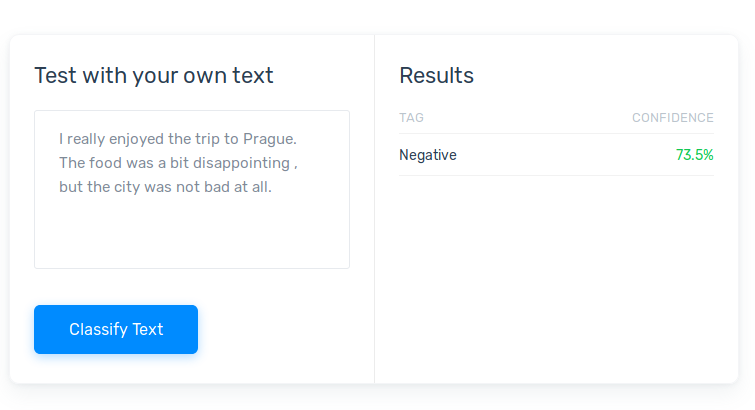
\includegraphics[width=0.7\textwidth]{figures/sentiment}
	\caption{Sentiment analysis example}
	\label{fig:sen}
\end{figure*}

Most commonly used methods:
\begin{itemize}
	\item \textbf{Rule-based}
	\item \textbf{Supervised methods} using training data, extracting features
	\item \textbf{Hybrid systems} combining the advantages of the rule based and the machine learning methods
\end{itemize}

\subsection{Question answering}
Question answering might be considered one of the oldest tasks in NLP or in AI in general with machine translation. With recent uprising products like Siri, Alexa, or Watson, it is still one of the most researched area.
If we build a question answering system, we need to take into consideration, that such system needs to handle factoid questions as well as complex request \cite{Ralph:2017}. If we want to process a factoid question such as \textit{What is the population of Europe?}, there is a clear criterion that we can define so the kind of a phrase that answers the question is clear, unlike non-factoid questions, where there may be many answers that satisfies the criterions, and sometimes it is unclear how many.

\begin{figure*}[h!]
	\centering
	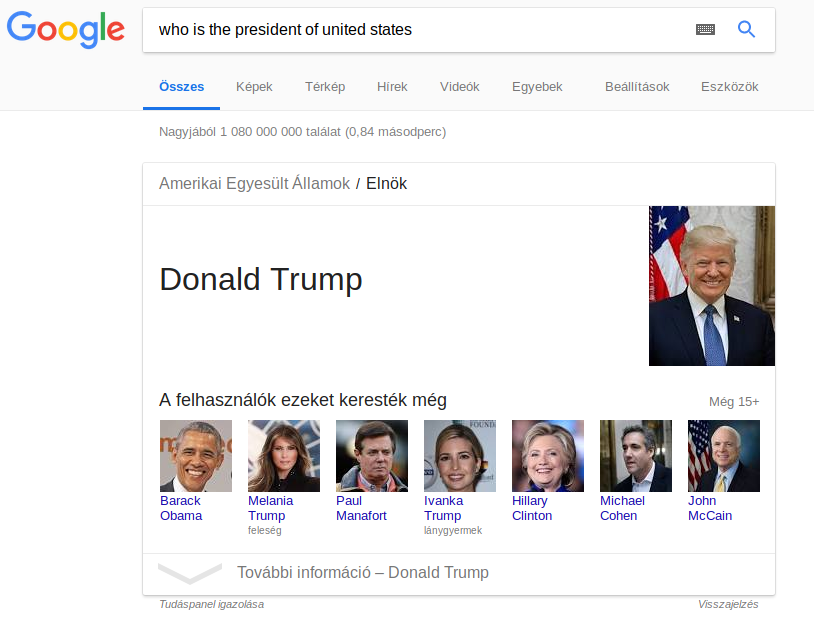
\includegraphics[width=0.7\textwidth]{figures/qagoogle}
	\caption{Question answering with google}
	\label{fig:qa}
\end{figure*}

Handling these types can be achieved using combinations of information retrieval (IR) and information extraction (IE) as described in \cite{Ralph:2017}.
IR based solutions is one of the major ones (e.g Google [\ref{fig:qa}], Watson). The main steps are:
\begin{itemize}
	\item detection the type of the questions
	\item building search queries
	\item retrieving ranked documents
	\item extracting relevant passages
	\item ranking answers
\end{itemize}

\begin{figure*}[h!]
	\centering
	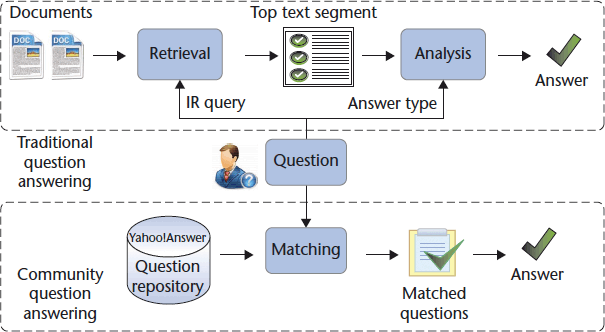
\includegraphics[width=0.7\textwidth]{figures/ie}
	\caption{Question processing system example \cite{IEsystem}}
	\label{fig:ie}
\end{figure*}

\section{Semantic parsing}
If we want to model the meaning of linguistic units, we need to map our data to some representation, so we need to choose a semantic representation. For syntactic analysis there are concepts, that are widely popular and accepted as a representation. But we cannot find such an agreement on what is the correct representation for semantic parsing.
Finding an absolute representation of semantics knowledge can be described as one of the most challenging AI task of our time, and if one could be able to construct such engine, it would be capable of \textbf{artificial general intelligence} \cite{Kornai:2018}, so we could essentially model the thinking of humans. Kornai summarized in \cite{Kornai:2018} what can be expected of a theory of semantics:
\begin{quotation}
	"our goal must be to develop a theory capable of handling the kind of commonsensical inferences that people routinely, automatically, and generally subconsciously make when answering simple questions about simple stories"
\end{quotation}

\subsection{Distributional models}
In the field of natural language processing one way of encoding semantic meaning is to use distributional models. In these models, two words are similar if they appear in the same context, and model semantic meaning as real-valued vectors. These vectors need to be constructed from a training data, and we can calculate similarity as euclidean distance between the vectors.

Lets have a look at these two sentences \textit{"The cat is walking in the bedroom"} and \textit{"A dog was running in a room"}. Words \textit{"dog"} and \textit{"cat"} have a similar semantic meaning, so if they are represented by vectors, which distance from each other is small, than we can vary the sentences \textit{"The dog is walking in the bedroom"} and \textit{"A cat was running in a room"} \cite{Bengio:2003}. The intuition is that these models want to obtain the meaning from the words around it \cite{Jurafsky:2018}. These meaning are represented by vectors, called embeddings. One of the first models build around these intuitions was introduced by Bengio \cite{Bengio:2003}. 

These word embeddings used in basically all state-of-the art systems related to natural language processing applications. Mikolov \cite{Mikolov:2013c} showed that words embeddings can be applied for vector operations, like addition or subtraction, and these operations often result in meaningful representation. Lets look at the example of vector("King") - vector("Man") + vector("Woman") \ref{fig:vecs} which results in vector("Queen"). While the usage of word embeddings brought an important breakthrough in modelling word meaning, applying them for bigger linguistics units like phrases, sentences or even whole text remained a difficult challenge even for nowadays. One of the biggest reasons for this is the additive aspect of these models: if we model A B C expression with vector v(A) + v(B) + v(C), then we represent "John killed Bill" and "Bill killed John" sentences in the same way. 

\begin{figure*}[h!]
	\centering
	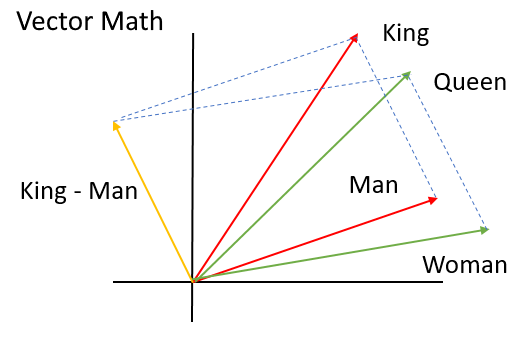
\includegraphics[width=0.7\textwidth]{figures/vecs}
	\caption{Vector addition example}
	\label{fig:vecs}
\end{figure*}

The other issue is that we know very little about the structure of a multi dimensional real-value vector (for embeddings it can be from 300 up to 1000 dimension), so it makes it very hard to understand why and when they work. So while most state-of-the art systems use word embeddings as a sole representation of meaning, and while it can be useful to encode meaning as vectors, so it can create connection from language specific and non-language specific data, we cannot deny the importance of having other semantics representations, such as graph-based ones. 

In the majority of our work, we researched graph-based solutions, where we model the meaning of lingustics unit with graphs, and the whole process can be defined with graph transformations. Next I will briefly introduce graph based formalism starting with Abstract Meaning Representations (AMR) followed by the introduction of the 4lang formalism, which will be the focus of the work, and I will go into the details in the next chapter.

\subsection{Abstract Meaning Representations}
Abstract Meaning Representation (AMR) was introduced by Banarescu\cite{Banarescu:2013} for representing the meaning of linguistic structures. They represent meaning as labeled, directed, acyclic graphs, that can be used to capture the meaning of whole sentences, so if two sentences are similar in meaning, they should be represented by similar graphs. In the past few years, we have seen multiple works related to AMR graphs, like an AMR-annotated corpus\cite{Banarescu:2013}, or multi-sentence AMR corpus \cite{OGorman2018AMRBT}, and various parsing applications \cite{DAC:2017} \cite{Vanderwende:2015}.

Nodes of AMR graphs can be represented various ways. Each node in the graph represents a semantic concept \cite{AMR:2015}, that can be either an English word, or frameset from PropBank \cite{Palmer:2005}, essentially used for abstraction. The framesets are English verbs. The AMR introduced these variables for entities, events, properties, and states. An AMR can be converted to multiple formats:
\begin{itemize}
	\item Logic format
	\item AMR format
	\item Graph format
	
	These formats can be seen on Figure \ref{fig:amr} for sentence \textit{"the boy wants to go"}, and the corresponding 4lang representation on Figure \ref{fig:4langboy}.
	
\end{itemize}

\begin{figure*}[h!]
	\centering
	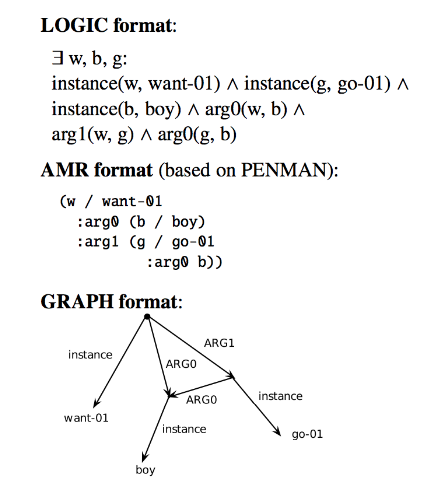
\includegraphics[height=0.4\textwidth]{figures/amr}
	\caption{Example sentence and representations}
	\label{fig:amr}
\end{figure*}

In this thesis we use the semantic parser 4lang \cite{Recski:2015b}, and unlike 4lang, AMR handles wider range of phenomenas, mostly typical of English, and AMR is not interlingua, it is heavily biased towards English \cite{Palmer:2005}, while 4lang can deal with multiple language.

\begin{figure*}[h!]
	\centering
	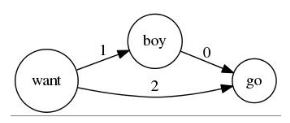
\includegraphics[width=0.3\textwidth]{figures/4langboy}
	\caption{Example sentence and representations in 4lang}
	\label{fig:4langboy}
\end{figure*}

In the next chapter, I will go into details about the 4lang formalism, and the parser itself. After I will describe our method of measuring similarities between semantic graphs, and its usage on semantic related tasks.